\documentclass[conference]{IEEEtran}
\IEEEoverridecommandlockouts
\usepackage{siunitx}
\usepackage{listings}
\usepackage{xcolor}
\usepackage{hyperref}
\usepackage{amsthm}
\usepackage{pgfplots}
\usepackage{graphicx}
\lstset { %
    language=Python,
    backgroundcolor=\color{black!5}, % set backgroundcolor
    basicstyle=\footnotesize,% basic font setting
}
%New colors defined below
\definecolor{codegreen}{rgb}{0,0.6,0}
\definecolor{codegray}{rgb}{0.5,0.5,0.5}
\definecolor{codepurple}{rgb}{0.58,0,0.82}
\definecolor{backcolour}{rgb}{0.95,0.95,0.92}

%Code listing style named "mystyle"
\lstdefinestyle{mystyle}{
  backgroundcolor=\color{backcolour},   commentstyle=\color{codegreen},
  keywordstyle=\color{magenta},
  numberstyle=\tiny\color{codegray},
  stringstyle=\color{codepurple},
  basicstyle=\ttfamily\footnotesize,
  breakatwhitespace=false,         
  breaklines=true,                 
  captionpos=b,                    
  keepspaces=true,                 
  numbers=left,                    
  numbersep=5pt,                  
  showspaces=false,                
  showstringspaces=false,
  showtabs=false,                  
  tabsize=2
}

%"mystyle" code listing set
\lstset{style=mystyle}
% The preceding line is only needed to identify funding in the first footnote. If that is unneeded, please comment it out.
\usepackage{cite}
\usepackage{amsmath,amssymb,amsfonts}
\usepackage{algorithmic}
\usepackage{graphicx}
\usepackage{textcomp}
\usepackage{xcolor}
\def\BibTeX{{\rm B\kern-.05em{\sc i\kern-.025em b}\kern-.08em
    T\kern-.1667em\lower.7ex\hbox{E}\kern-.125emX}}
\begin{document}

\title{DAA Assignment-06\\
}

\author{\IEEEauthorblockN{ Ayush Khandelwal }
\IEEEauthorblockA{\textit{IIT2019240} \\
}
\and
\IEEEauthorblockN{Ayush Bhagta}
\IEEEauthorblockA{\textit{IIT2019501} \\
}
\and
\IEEEauthorblockN{Tauhid Alam}
\IEEEauthorblockA{\textit{BIM2015003} \\
}
}

\maketitle

\begin{abstract}
In this report we designed a Breath first search in graph algorithm to find minimum steps through which we can reach from initial state i.e both jugs empty
to a final state where one of the jugs has a given quantity of water d in litres.

\end{abstract}

\section{Introduction}
Given a m liter jug and a n liter jug which are initially empty. The jugs don’t have markings to allow measuring smaller quantities. We have to use the jugs to measure d liters of water where d $<$ n and d $<$ m.

(X, Y) corresponds to a state where X refers to amount of water in Jug1 and Y refers to amount of water in Jug2 
Determine the path from initial state (xi, yi) to final state (xf, yf), where (xi, yi) is (0, 0) which indicates both Jugs are initially empty and (xf, yf) indicates a state which could be (0, d) or (d, 0).

The operations you can perform are: 
\begin{itemize}
\item Empty a Jug, (X, Y)$->$(0, Y) Empty Jug 1
\item Fill a Jug, (0, 0)-$>$(X, 0) Fill Jug 1
\item Pour water from one jug to the other until one of the jugs is either empty or full, (X, Y) -> (X-d, Y+d)
\end{itemize}
Breadth-first search is an algorithm for traversing or searching tree or graph data structures. It starts at the tree root, and explores all of the neighbor nodes at the present depth prior to moving on to the nodes at the next depth level.
We run breadth first search on the states and these states will be created after applying allowed operations and we also use visited map of pair to keep track of states that should be visited only once in the search. This solution can also be achieved using depth first search.


\section{Algorithm Design}
\textbf{Brute Force :}\\*
The  associated  Diophantine  equation  of the  problem  is given  by  $mx+ny=d$, whose  solution is described  by  the theorem below.\\
\underline{Theorem}. \\
The Diophantine equation $mx+ny=d$ is solvable if and only if gcd(m, n) divides d. For convenience,  let  us  assume  $mx+ny=d$  is  solvable  in  the discussions below. Depending on which jug is chosen to be filled first, there are two possible solutions for solving the two water jugs problems. They are labelled by M1 and M2 in the following algorithms:\\ 
\underline{Algorithm}.\\
Input: The integers m, n and d, where 0$<$m$<$n and d$<$n.  \\
Output:  An  integer  sequence  corresponding  to  a  feasible solution (called M1) of the two water jugs problem, by filling the m-litre jug first. \\
Procedure:
Step 1. Initialize a dummy variable k = 0.\\
Step 2. If k $<$ d, then repeat adding m to k and assign the result to k until k = d or k $>$ n.\\
Step 3. If k $>$ n, then subtract n from k and assign the result to k.\\
Step 4. If k = d, then stop. Otherwise, repeat the steps from Step 2 to Step 4. The number of additions  (say x1) and subtractions (say  y1) involved  provides a  solution  to  the  Diophantine  equation mx+ny=d, namely x = x1, y = -y1. The actual pouring sequence can  be  determined  by  referring  to  the  integer  sequence obtained.  \\
Algorithm 2.2.\\
Input: The integers m, n and d, where 0<m<n and d<n.  \\
Output:  An  integer  sequence  corresponding  to  a  feasible solution (called M2) of the two water jugs problem, by filling the n-litre jug first.\\
Procedure: \\
Step 1. Initialize a dummy variable k = 0. \\
Step 2. If k = d, then add n to k and assign the result to k. \\
Step 3. If k $>$ d, then repeat subtracting m from k and assign the result to k until k $=$ d or k $<$ m.  \\
Step 4. If k = d, then stop. Otherwise, repeat the steps from Step 2 to Step 4. The number of subtractions  (say x2)  and additions (say y2) involved  provides a  solution  to  the  Diophantine  equation mx+ny$=$d, namely x = -x2, y = y2. The actual pouring sequence can  be  determined  by  referring  to  the  integer  sequence obtained.\\

  

\textbf{Using Graph :}


Step 1. Initialize an empty sting of pair containing [0,0] that is the initial state of the jugs. This string contain path for a particular state to be achieved. \\

Step 2. We Initialize an empty deque(Doubly Ended Queue) and push the first path that is [[0,0]] to it.  \\

Step 3. We check if last state of the the left most path of the deque is the required path or not and exit the loop and save that path in the final path variable and move to Step6 if the condition satisfies. Otherwise continue to Step 4.\\

Step 4. We look for all the possible cases from the last state of the first path that is in the queue and remove that path and further add all the possible paths to the queue to left for the DFS(Depth First Search) approach or to the right for BFS(Breadth First Search) approach.\\

Step 5.We go back to step 3 and continue the iteration until no further transition is possible that is the given condition could not be satisfied.\\

Step 6. We print the final path variable in the order of transitions made to reach the condition.\\


\section{Algorithm and illustration}
\textbf{Brute-Force}\\
Volume of first jug: 3\\
Volume of second jug: 4\\
Desired volume: 2\\
k=0\\
Repeat adding 3 to k until k=2 or k>4\\
k=3+3=6\\
Now subtract 4 from k\\
k=6-4=2\\
As k= desired volume so we stop here.\\
The actual pouring sequence can be determined by referring to the integer sequence obtained.
[0,0][0,3][3,0][3,3][2,4]
\\ \\
\textbf{Using Graph}:\\
BFS:\\
Volume of first jug: 5\\
Volume of second jug: 4\\
Desired volume: 2\\\
First we append {0,0} to our path\\
path={[0,0]}\\
Now next possible transitions from [0,0] are [5,0] [0,4]\\
next={[0,4],[5,0]}\\
Now next possible transitions from [5,0] are [5,4] [1,4]\\
next={[0,4],[5,4],[1,4]}\\
Now next possible transitions from [0,4] are [5,4] [4,0]\\
next={[5,4],[1,4],[5,4],[4,0]}\\
Now next possible transitions from [5,4] are [no more transitions]:\\
next={[1,4],[5,4],[4,0]}\\
Now next possible transitions from [1,4] are [1,0]:\\
next={[5,4],[4,0],[1,0]}\\
Now next possible transitions from [5,4] are [no more transitions]:\\
next={[4,0],[1,0]}\\
Now next possible transitions from [4,0] are [4,4]:\\
next={[1,0],[4,4]}\\
Now next possible transitions from [1,0] are [0,1]:\\
next={[4,4],[0,1]}\\
Now next possible transitions from [4,4] are [5,3]:\\
next={[0,1],[5,3]}\\
Now next possible transitions from [0,1] are [5,1]:\\
next={[5,3],[5,1]}\\
Now next possible transitions from [5,3] are [0,3]:\\
next={[5,1],[0,3]}\\
Now next possible transitions from [5,1] are [2,4]:\\
next={[0,3],[2,4]}\\
Now next possible transitions from [0,3] are [3,0]:\\
next={[2,4][3,0]}\\
Now next possible transitions from [2,4] are [2,0]:\\
Goal is achieved as we have [2,0] as a state\\
Now path=[0,0] [5,0] [1,4] [1,0] [0,1] [5,1] [2,4]\\\\
\\
DFS:\\
Volume of first jug: 4\\
Volume of second jug: 3\\
Desired volume: 2\\\
First we append {0,0} to our path\\
path={[0,0]}\\
Now next possible transitions from [0,0] are [4,0] [0,3]\\
next={[0,3],[4,0]}\\
Now next possible transitions from [0,3] are [4,3] [3,0]\\
next={[3,0],[4,3],[4,0]}\\
Now next possible transitions from [3,0] are [4,0] [3,3]\\
next={[3,3],[4,0],[4,3][4,0]}\\
Now next possible transitions from [3,3] are [4,3] [4,2]\\
next={[4,2],[4,3],[4,0],[4,3][4,0]}\\
Now next possible transitions from [4,2] are [0,2]\\
Goal achieved as we have 2 litres in one jug\\
Now Path={[0,0],[0,3],[3,0],[3,3][4,2]}\\

\section{Algorithm Analysis}
\textbf{Time complexity:}\\

\textbf{\underline{Using  Graph}}:\\
In this  approach we iterate over whole map generated by the nodes containing all the possible amount of water in both the jugs until we find the any of teh one required condition. So to iterate over a graph by BFS or by DFS time complexity will be as below:\\

\underline{Best Case}-If the required amount of water is equal to capacity of one of the jug.This will result in the time complexity of constant order.So\\ \textit{\textbf{Best Case Time Complexity= \si{\ohm}(1)}}

\underline{Worst Case}-If the given condition is true and the required amount of water is what we get at the farthest end.This will result in the time complexity of order $O(V+E)$ where E ranges from 1 to $V^{2}$, but in our case number of edges is equal to six hence number of edges will be of order $3V$, so, the time complexity will be of order 4V, which is treated as linear in time complexity, where V is the number of nodes and E is the number of Edges. Maximum value of V in this case could be N*M where N and M are the maximum capacities of mug.So \\\textit{\textbf{Worst Case Time Complexity=O($V$)= O($N*M$)}}\\\\


 \begin{center}
 \begin{tabular}{||c| c| c||} 
 \hline
 N & M & Time(in nanoseconds) \\ [0.5ex] 
 \hline\hline
 7 & 19 & 6198  \\ 
 \hline
 37 & 29 & 92824  \\ 
 \hline
 107 & 23 & 92983 \\ 
 \hline
 347 & 31 & 249966  \\ 
 \hline
 457 & 37 & 167850  \\ 
 \hline
 659 & 53 & 528953  \\ 
 \hline
 1487 & 31 & 4728464  \\ 
 \hline
 3109 & 31 & 10779433  \\ [1ex] 
  \hline
\end{tabular}
\end{center}

\begin{figure}[h]
\caption{Graph of Time of Execution (in nanoseconds ) Against $N*M$}
\centering
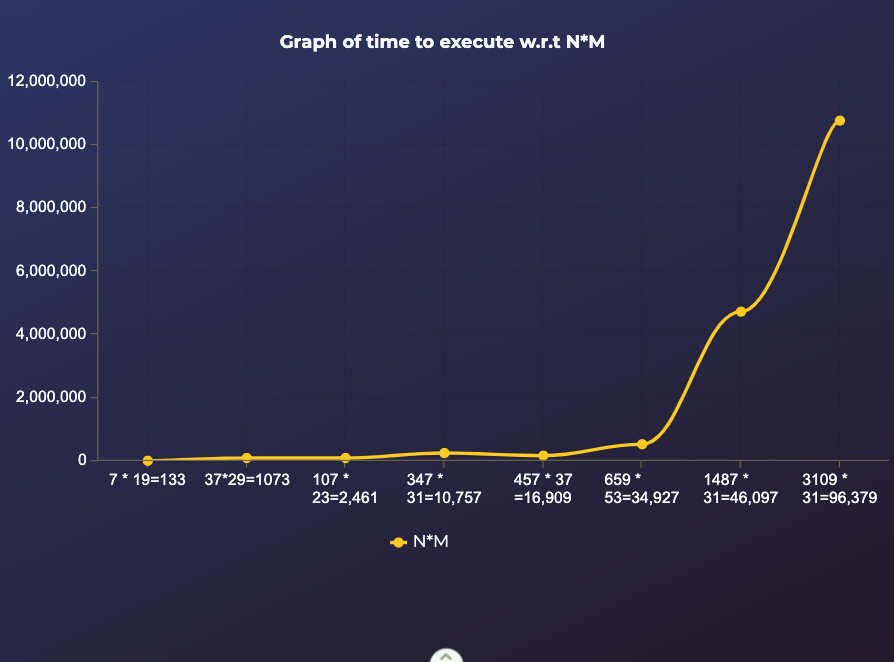
\includegraphics[width=8cm]{images/graphs.jpg}
\end{figure}


\textbf{Space complexity:}\\
\underline{Brute-Force}:\\
In Brute force we will be directly adding and subtracting in an integer so no extra space is required .\\
This will result in the space complexity of $O(1)$. 
\\\\\\
\underline{Using  Graph}:\\
In this  approach we don't have need to store any graph as all the path are logically decided and checked at the time, so no more Extra space is required to store the map.But we store the path that is used to reach that point which whose length vary from 1 to V and we need to store path for all V vertices and hence the required space is of order $V^{2}$.  Maximum value of V in this case could be N*M where N and M are the maximum capacities of mug.So \textit{\textbf{Space Complexity= O($(N*M)^{2}$)}}\\\\


\section{Conclusion}
We can observe that in graph the space required is more but it is much more efficient in terms of time and will be favourable for the values having bigger differences in the capacity of jugs.

 \section{References}
 \begin{enumerate}
\color{blue}
\item \url{https://www.geeksforgeeks.org/breadth-first-search-or-bfs-for-a-graph/} 
\item \url{https://www.geeksforgeeks.org/depth-first-search-or-dfs-for-a-graph/}
\item \url{https://www.eecis.udel.edu/~mccoy/courses/cisc4-681.10f/lec-materials/handouts/search-water-jug-handout.pdf}
\item \url{https://en.wikipedia.org/wiki/Breadth-first_search}
\item \url{https://en.wikipedia.org/wiki/Depth-first_search}
\item R.  S.  Mary,  “An  alternative  arithmetic  approach  to  the  water  jugs problem,”  Proceedings  on National  Conference  on  Computational Intelligence for Engineering Quality Software, 1, 2014, pp. 10-13.
\item S.  Abu  Naser,  “Developing  visualization  tool  for  the  teaching  AI searching algorithms,” Information Technology Journal,  7(2), 2008, pp. 350–355. 
 \end{enumerate}
\color{black}
\
\begin{titlepage}
    \begin{center}
        \Huge
        \section*{Appendix}
        \end{center}
         \textbf{Code for implementation of this paper is given below:}
\begin{lstlisting}[language=Python,caption=Code for this paper]
import collections

"""
Authors: Ayush Khandelwal IIT2019240
         Ayush Bhagta    IIT2019501
         Tauhid Alam    BIM2015003
States:  Amount of water in each respective jug, where the states are represented by
            [a, b] and a is the amount in the first jug and b is the amount in the second jug
Initial State: [0,0]
Goal state: either of the jugs contains the amount of water inputted by the user
Operators:  1. Fill the first jug   
            2. Fill the second jug  
            3. Empty the first jug
            4. Empty the second jug
            5. Pour the first jug into the second jug
            6. Pour the second jug into the second jug
Branching Factor:   6 (because we have 6 operators)
"""


def main():
    """
    main function
    """

    starting_node = [[0, 0]]
    jugs = get_jugs()
    goal_amount = get_goal(jugs)
    check_dict = {}
    is_depth = get_search_type()
    search(starting_node, jugs, goal_amount, check_dict, is_depth)

def get_index(node):
    """
    returns a key value for a given node
    
    node: a list of two integers representing current state of the jugs 
    """
    return pow(7, node[0]) * pow(5, node[1])


def get_search_type():
    """
    Returns True for DFS, False otherwise.
    """
    
    s = input("Enter 'b' for BFS, 'd' for DFS: ")
    s = s[0].lower()
    
    while s != 'd' and s != 'b':
        s = input("The input is not valid! Enter 'b' for BFS, 'd' for DFS: ")
        s = s[0].lower()
        
    return s == 'd'

def get_jugs():
    """
    Returns a list of two integeres representing volumes of the jugs.
    Takes volumes of the jugs as an input from the user.
    """
    print("Receiving the volume of the jugs...")
    jugs = []
    
    temp = int(input("Enter first jug volume (>1): "))
    while temp < 1:
        temp = int(input("Enter a valid amount (>1): "))       
    jugs.append(temp)
    
    temp = int(input("Enter second jug volume (>1): "))
    while temp < 1:
        temp = int(input("Enter a valid amount (>1): "))     
    jugs.append(temp)
    
    return jugs

def get_goal(jugs):
    """
    Returns desired amount of water.
    Takes desired amount as an input from the user.
    
    jugs: a list of two integers representing volumes of the jugs
    """

    print("Receiving the desired amount of the water...")

    max_amount = max(jugs[0], jugs[1])
    s = "Enter the desired amount of water (1 - {0}): ".format(max_amount)
    goal_amount = int(input(s))
    while goal_amount < 1 or goal_amount > max_amount:
        goal_amount = int(input("Enter a valid amount (1 - {0}): ".format(max_amount)))
        
    return goal_amount

def is_goal(path, goal_amount):
    """
    Returns True, if the given path terminates at the goal node.
    
    path: a list of nodes representing the path to be checked
    goal_amount: an integer representing the desired amount of water
    """

    print("Checking if the gaol is achieved...")
    
    return path[-1][0] == goal_amount or path[-1][1] == goal_amount

def been_there(node, check_dict):
    """
    Returns True, if the given node is already visited
    
    node: a list of two integers representing current state of the jugs
    check_dict: a dictionary storing visited nodes
    """

    print("Checking if {0} is visited before...".format(node))

    return check_dict.get(get_index(node), False)

def next_transitions(jugs, path, check_dict):
    """
    Returns list of all possible transitions whcih do not cause loops
    
    jugs: a list of two integers representing volumes of the jugs
    path: a list of nodes represeting the current path
    check_dict: a dictionary storing visited nodes
    """

    print("Finding next transitions and checking for the loops...")
    
    result = []
    next_nodes = []
    node = []
    
    a_max = jugs[0]
    b_max = jugs[1]
    
    a = path[-1][0]  # initial amount in the first jug
    b = path[-1][1]  # initial amount in the second jug

    # 1. fill in the first jug
    node.append(a_max)
    node.append(b)
    if not been_there(node, check_dict):
        next_nodes.append(node)
    node = []

    # 2. fill in the second jug
    node.append(a)
    node.append(b_max)
    if not been_there(node, check_dict):
        next_nodes.append(node)
    node = []

    # 3. second jug to first jug
    node.append(min(a_max, a + b))
    node.append(b - (node[0] - a))  # b - ( a' - a)
    if not been_there(node, check_dict):
        next_nodes.append(node)
    node = []

    # 4. first jug to second jug
    node.append(min(a + b, b_max))
    node.insert(0, a - (node[0] - b))
    if not been_there(node, check_dict):
        next_nodes.append(node)
    node = []

    # 5. empty first jug
    node.append(0)
    node.append(b)
    if not been_there(node, check_dict):
        next_nodes.append(node)
    node = []

    # 6. empty second jug
    node.append(a)
    node.append(0)
    if not been_there(node, check_dict):
        next_nodes.append(node)

    # create a list of next paths
    for i in range(0, len(next_nodes)):
        temp = list(path)
        temp.append(next_nodes[i])
        result.append(temp)

    if len(next_nodes) == 0:
        print("No more unvisited nodes...\nBacktracking...")
    else:
        print("Possible transitions: ")
        for nnode in next_nodes:
            print(nnode)

    return result


def transition(old, new, jugs):
    """
    returns a string explaining the transition from old state/node to new state/node
    
    old: a list representing old state/node
    new: a list representing new state/node
    jugs: a list of two integers representing volumes of the jugs
    """
    
    a = old[0]
    b = old[1]
    a_prime = new[0]
    b_prime = new[1]
    a_max = jugs[0]
    b_max = jugs[1]

    if a > a_prime:
        if b == b_prime:
            return "Clear {0}-liter jug:\t\t\t".format(a_max)
        else:
            return "Pour {0}-liter jug into {1}-liter jug:\t".format(a_max, b_max)
    else:
        if b > b_prime:
            if a == a_prime:
                return "Clear {0}-liter jug:\t\t\t".format(b_max)
            else:
                return "Pour {0}-liter jug into {1}-liter jug:\t".format(b_max, a_max)
        else:
            if a == a_prime:
                return "Fill {0}-liter jug:\t\t\t".format(b_max)
            else:
                return "Fill {0}-liter jug:\t\t\t".format(a_max)


def print_path(path, jugs):
    """
    prints the goal path
    
    path: a list of nodes representing the goal path
    jugs: a list of two integers representing volumes of the jugs
    """
    
    print("Starting from:\t\t\t\t", path[0])
    for i in  range(0, len(path) - 1):
        print(i+1,":", transition(path[i], path[i+1], jugs), path[i+1])

def search(starting_node, jugs, goal_amount, check_dict, is_depth):
    """
    searchs for a path between starting node and goal node
    
    starting_node: a list of list of two integers representing initial state of the jugs
    jugs: a list of two integers representing volumes of the jugs
    goal_amount: an integer represting the desired amount
    check_dict: a dictionary storing visited nodes
    is_depth: implements DFS, if True; BFS otherwise
    """

    if is_depth:
        print("Implementing DFS...")
    else:
        print("Implementing BFS...")

    goal = []
    accomplished = False
    
    q = collections.deque()
    q.appendleft(starting_node)
    
    while len(q) != 0:
        path = q.popleft()
        check_dict[get_index(path[-1])] = True
        if len(path) >= 2:
            print(transition(path[-2], path[-1], jugs), path[-1])
        if is_goal(path, goal_amount):
            accomplished = True
            goal = path
            break

        next_moves = next_transitions(jugs, path, check_dict)
        for i in next_moves:
            if is_depth:
                q.appendleft(i)
            else:
                q.append(i)

    if accomplished:
        print("The goal is achieved\nPrinting the sequence of the moves...\n")
        print_path(goal, jugs)
    else:
        print("Problem cannot be solved.")


if __name__ == '__main__':
    main()
\end{lstlisting}
\end{titlepage}
\end{document}
